\documentclass{article}

\def\npart {IA}
\def\nterm {Michaelmas}
\def\nyear {2023}
\def\nlecturer {Prof H.\ Winton}
\def\ncourse {Groups}

\usepackage{alltt}
\usepackage{amsmath, amsfonts, amssymb, amsthm}
\usepackage{booktabs}
\usepackage{caption}
\usepackage{enumitem}
\usepackage{fancyhdr}
\usepackage{graphicx}
\usepackage{mathdots}
\usepackage{mathtools}
\usepackage{microtype}
\usepackage{multirow}
\usepackage{pdflscape}
\usepackage{pgfplots}
\usepackage{siunitx}
\usepackage{textcomp}
\usepackage{slashed}
\usepackage{tabularx}
\usepackage{tikz}
\usepackage{tkz-euclide}
\usepackage[normalem]{ulem}
\usepackage[all]{xy}

\pgfplotsset{compat=1.18}
\pagestyle{fancyplain}

\lhead{\emph{\nouppercase{\leftmark}}}
\rhead{
  \ifnum\thepage=1
  \else
    \npart\ \vline\ \ncourse
  \fi}

\def\nauthor{Marcus Ng}
\author{Based on lectures by \nlecturer \\\small Notes taken by \nauthor}
\date{\nterm\ \nyear}
\title{Part \npart\ --- \ncourse}

\newcommand*{\Cdot}{{\raisebox{-0.25ex}{\scalebox{1.5}{$\cdot$}}}}
\setlist[enumerate,1]{label={(\roman*)}}

\newcommand {\pd}[2][ ]{
  \ifx #1 { }
    \frac{\partial}{\partial #2}
  \else
    \frac{\partial^{#1}}{\partial #2^{#1}}
  \fi
}

% Theorems
\theoremstyle{definition}
\newtheorem*{aim}{Aim}
\newtheorem*{axiom}{Axiom}
\newtheorem*{claim}{Claim}
\newtheorem*{cor}{Corollary}
\newtheorem*{conjecture}{Conjecture}
\newtheorem*{defi}{Definition}
\newtheorem*{eg}{Example}
\newtheorem*{ex}{Exercise}
\newtheorem*{fact}{Fact}
\newtheorem*{law}{Law}
\newtheorem*{lemma}{Lemma}
\newtheorem*{notation}{Notation}
\newtheorem*{prop}{Proposition}
\newtheorem*{question}{Question}
\newtheorem*{problem}{Problem}
\newtheorem*{rrule}{Rule}
\newtheorem*{thm}{Theorem}
\newtheorem*{assumption}{Assumption}
\newtheorem*{assert}{Assertion}

\newtheorem*{remark}{Remark}
\newtheorem*{warning}{Warning}
\newtheorem*{exercise}{Exercise}

\newtheorem{nthm}{Theorem}[section]
\newtheorem{nlemma}[nthm]{Lemma}
\newtheorem{nprop}[nthm]{Proposition}
\newtheorem{ncor}[nthm]{Corollary}

\SetEnumitemKey{cases}{
  label=\underline{Case~\arabic*:},
  ref={\arabic*},
  align=left,
  leftmargin=\parindent
}

% \renewcommand{\labelitemi}{--}
% \renewcommand{\labelitemii}{$\circ$}
% \renewcommand{\labelenumi}{(\roman{*})}

\let\stdsection\section
\renewcommand\section{\newpage\stdsection}

% Strike through
\def\st{\bgroup \ULdepth=-.55ex \ULset}


%%%%%%%%%%%%%%%%%%%%%%%%%
%%%%% Maths Symbols %%%%%
%%%%%%%%%%%%%%%%%%%%%%%%%

% Logical symbols
\newcommand{\contradiction}{
  
\begin{tikzpicture}[rotate=45,x=0.5ex,y=0.5ex]
  \draw[line width=.1ex] (0,2) -- (3,2) (0,1) -- (3,1) (1,3) -- (1,0) (2,3) -- (2,0);
  \end{tikzpicture}
}


\let\U\relax
\let\C\relax
\let\G\relax

% Matrix groups
% \newcommand{\GL}{\mathrm{GL}}
% \newcommand{\Or}{\mathrm{O}}
% \newcommand{\PGL}{\mathrm{PGL}}
% \newcommand{\PSL}{\mathrm{PSL}}
% \newcommand{\PSO}{\mathrm{PSO}}
% \newcommand{\PSU}{\mathrm{PSU}}
% \newcommand{\SL}{\mathrm{SL}}
% \newcommand{\SO}{\mathrm{SO}}
% \newcommand{\Spin}{\mathrm{Spin}}
% \newcommand{\Sp}{\mathrm{Sp}}
% \newcommand{\SU}{\mathrm{SU}}
\newcommand{\U}{\mathrm{U}}
% \newcommand{\Mat}{\mathrm{Mat}}

% Matrix algebras
% \newcommand{\gl}{\mathfrak{gl}}
% \newcommand{\ort}{\mathfrak{o}}
% \newcommand{\so}{\mathfrak{so}}
% \newcommand{\su}{\mathfrak{su}}
% \newcommand{\uu}{\mathfrak{u}}
% \renewcommand{\sl}{\mathfrak{sl}}

% Special sets
\newcommand{\C}{\mathbb{C}}
\newcommand{\CP}{\mathbb{CP}}
\newcommand{\GG}{\mathbb{G}}
\newcommand{\N}{\mathbb{N}}
\newcommand{\Q}{\mathbb{Q}}
\newcommand{\R}{\mathbb{R}}
\newcommand{\RP}{\mathbb{RP}}
\newcommand{\T}{\mathbb{T}}
\newcommand{\Z}{\mathbb{Z}}
\renewcommand{\H}{\mathbb{H}}

% Brackets
\newcommand{\abs}[1]{\left\lvert #1\right\rvert}
\newcommand{\bket}[1]{\left\lvert #1\right\rangle}
\newcommand{\brak}[1]{\left\langle #1 \right\rvert}
\newcommand{\braket}[2]{\left\langle #1\middle\vert #2 \right\rangle}
\newcommand{\bra}{\langle}
\newcommand{\ket}{\rangle}
\newcommand{\norm}[1]{\left\lVert #1\right\rVert}
\newcommand{\normalorder}[1]{\mathop{:}\nolimits\!#1\!\mathop{:}\nolimits}
\newcommand{\tv}[1]{|#1|}
\renewcommand{\vec}[1]{\boldsymbol{\mathbf{#1}}}

% not-math
% \newcommand{\bolds}[1]{{\bfseries #1}}
% \newcommand{\cat}[1]{\mathsf{#1}}
% \newcommand{\ph}{\,\cdot\,}
% \newcommand{\term}[1]{\emph{#1}\index{#1}}
% \newcommand{\phantomeq}{\hphantom{{}={}}}

% Probability
% \DeclareMathOperator{\Bernoulli}{Bernoulli}
% \DeclareMathOperator{\betaD}{beta}
% \DeclareMathOperator{\bias}{bias}
% \DeclareMathOperator{\binomial}{binomial}
% \DeclareMathOperator{\corr}{corr}
% \DeclareMathOperator{\cov}{cov}
% \DeclareMathOperator{\gammaD}{gamma}
% \DeclareMathOperator{\mse}{mse}
% \DeclareMathOperator{\multinomial}{multinomial}
% \DeclareMathOperator{\Poisson}{Poisson}
% \DeclareMathOperator{\var}{var}
% \newcommand{\E}{\mathbb{E}}
% \newcommand{\Prob}{\mathbb{P}}

% Algebra
% \DeclareMathOperator{\adj}{adj}
% \DeclareMathOperator{\Ann}{Ann}
% \DeclareMathOperator{\Aut}{Aut}
% \DeclareMathOperator{\Char}{char}
% \DeclareMathOperator{\disc}{disc}
% \DeclareMathOperator{\dom}{dom}
% \DeclareMathOperator{\fix}{fix}
% \DeclareMathOperator{\Hom}{Hom}
% \DeclareMathOperator{\id}{id}
% \DeclareMathOperator{\image}{image}
% \DeclareMathOperator{\im}{im}
% \DeclareMathOperator{\re}{re}
% \DeclareMathOperator{\tr}{tr}
% \DeclareMathOperator{\Tr}{Tr}
% \newcommand{\Bilin}{\mathrm{Bilin}}
% \newcommand{\Frob}{\mathrm{Frob}}

% Others
% \newcommand\ad{\mathrm{ad}}
% \newcommand\Art{\mathrm{Art}}
% \newcommand{\B}{\mathcal{B}}
% \newcommand{\cU}{\mathcal{U}}
% \newcommand{\Der}{\mathrm{Der}}
% \newcommand{\D}{\mathrm{D}}
% \newcommand{\dR}{\mathrm{dR}}
% \newcommand{\exterior}{\mathchoice{{\textstyle\bigwedge}}{{\bigwedge}}{{\textstyle\wedge}}{{\scriptstyle\wedge}}}
% \newcommand{\F}{\mathbb{F}}
% \newcommand{\G}{\mathcal{G}}
% \newcommand{\Gr}{\mathrm{Gr}}
% \newcommand{\haut}{\mathrm{ht}}
% \newcommand{\Hol}{\mathrm{Hol}}
% \newcommand{\hol}{\mathfrak{hol}}
% \newcommand{\Id}{\mathrm{Id}}
% \newcommand{\lie}[1]{\mathfrak{#1}}
% \newcommand{\op}{\mathrm{op}}
% \newcommand{\Oc}{\mathcal{O}}
% \newcommand{\pr}{\mathrm{pr}}
% \newcommand{\Ps}{\mathcal{P}}
% \newcommand{\pt}{\mathrm{pt}}
% \newcommand{\qeq}{\mathrel{``{=}"}}
% \newcommand{\Rs}{\mathcal{R}}
% \newcommand{\Vect}{\mathrm{Vect}}
% \newcommand{\wsto}{\stackrel{\mathrm{w}^*}{\to}}
% \newcommand{\wt}{\mathrm{wt}}
% \newcommand{\wto}{\stackrel{\mathrm{w}}{\to}}
% \renewcommand{\d}{\mathrm{d}}
% \renewcommand{\P}{\mathbb{P}}
%\renewcommand{\F}{\mathcal{F}}

\let\Im\relax
\let\Re\relax

% \DeclareMathOperator{\area}{area}
% \DeclareMathOperator{\card}{card}
% \DeclareMathOperator{\ccl}{ccl}
% \DeclareMathOperator{\ch}{ch}
% \DeclareMathOperator{\cl}{cl}
% \DeclareMathOperator{\cls}{\overline{\mathrm{span}}}
% \DeclareMathOperator{\coker}{coker}
% \DeclareMathOperator{\conv}{conv}
% \DeclareMathOperator{\cosec}{cosec}
% \DeclareMathOperator{\cosech}{cosech}
% \DeclareMathOperator{\covol}{covol}
% \DeclareMathOperator{\diag}{diag}
% \DeclareMathOperator{\diam}{diam}
% \DeclareMathOperator{\Diff}{Diff}
% \DeclareMathOperator{\End}{End}
% \DeclareMathOperator{\energy}{energy}
% \DeclareMathOperator{\erfc}{erfc}
% \DeclareMathOperator{\erf}{erf}
% \DeclareMathOperator*{\esssup}{ess\,sup}
% \DeclareMathOperator{\ev}{ev}
% \DeclareMathOperator{\Ext}{Ext}
% \DeclareMathOperator{\fst}{fst}
% \DeclareMathOperator{\Fit}{Fit}
% \DeclareMathOperator{\Frac}{Frac}
% \DeclareMathOperator{\Gal}{Gal}
% \DeclareMathOperator{\gr}{gr}
% \DeclareMathOperator{\hcf}{hcf}
\DeclareMathOperator{\Im}{Im}
% \DeclareMathOperator{\Ind}{Ind}
% \DeclareMathOperator{\Int}{Int}
% \DeclareMathOperator{\Isom}{Isom}
% \DeclareMathOperator{\lcm}{lcm}
% \DeclareMathOperator{\length}{length}
% \DeclareMathOperator{\Lie}{Lie}
% \DeclareMathOperator{\like}{like}
% \DeclareMathOperator{\Lk}{Lk}
% \DeclareMathOperator{\Maps}{Maps}
% \DeclareMathOperator{\orb}{orb}
% \DeclareMathOperator{\ord}{ord}
% \DeclareMathOperator{\otp}{otp}
% \DeclareMathOperator{\poly}{poly}
% \DeclareMathOperator{\rank}{rank}
% \DeclareMathOperator{\rel}{rel}
% \DeclareMathOperator{\Rad}{Rad}
\DeclareMathOperator{\Re}{Re}
% \DeclareMathOperator*{\res}{res}
% \DeclareMathOperator{\Res}{Res}
% \DeclareMathOperator{\Ric}{Ric}
% \DeclareMathOperator{\rk}{rk}
% \DeclareMathOperator{\Rees}{Rees}
% \DeclareMathOperator{\Root}{Root}
% \DeclareMathOperator{\sech}{sech}
% \DeclareMathOperator{\sgn}{sgn}
% \DeclareMathOperator{\snd}{snd}
% \DeclareMathOperator{\Spec}{Spec}
% \DeclareMathOperator{\spn}{span}
% \DeclareMathOperator{\stab}{stab}
% \DeclareMathOperator{\St}{St}
% \DeclareMathOperator{\supp}{supp}
% \DeclareMathOperator{\Syl}{Syl}
% \DeclareMathOperator{\Sym}{Sym}
% \DeclareMathOperator{\vol}{vol}

\begin{document}
\maketitle{
    \small
    \noindent\textbf{Examples of groups}\\
    Axioms for groups. Examples from geometry: symmetry groups of regular polygons, cube, tetrahedron. Permutations on a set; the symmetric group. Subgroups and homomorphisms. Symmetry groups as subgroups of general permutation groups. The M\"obius group; cross-ratios, preservation of circles, the point at infinity. Conjugation. Fixed points of M\"obius maps and iteration.\hspace*{\fill} [4]

    \vspace{10pt}
    \noindent\textbf{Lagrange's theorem}\\
    Cosets. Lagrange's theorem. Groups of small order (up to order 8). Quaternions. Fermat-Euler theorem from the group-theoretic point of view.\hspace*{\fill} [5]

    \vspace{10pt}
    \noindent\textbf{Group actions}\\
    Group actions; orbits and stabilizers. Orbit-stabilizer theorem. Cayley's theorem (every group is isomorphic to a subgroup of a permutation group). Conjugacy classes. Cauchy's theorem.\hspace*{\fill} [4]

    \vspace{10pt}
    \noindent\textbf{Quotient groups}\\
    Normal subgroups, quotient groups and the isomorphism theorem.\hspace*{\fill} [4]

    \vspace{10pt}
    \noindent
    \textbf{Matrix groups}\\
    The general and special linear groups; relation with the M\"obius group. The orthogonal and special orthogonal groups. Proof (in $\R^3$) that every element of the orthogonal group is the product of reflections and every rotation in $\R^3$ has an axis. Basis change as an example of conjugation.\hspace*{\fill} [3]
    
    \vspace{10pt}
    \noindent\textbf{Permutations}\\
    Permutations, cycles and transpositions. The sign of a permutation. Conjugacy in $S_n$ and in $A_n$. Simple groups; simplicity of $A_5$.\hspace*{\fill} [4]}
    
\tableofcontents

%%%%%%%%%%%%%%%%%%%%%%
% Lecture 1: 5/10/2023
%%%%%%%%%%%%%%%%%%%%%%

\section{Examples and Definitions}

There are two ways of looking at groups; an algebraic approach that deals with equations and variables, and a geometric approach that looks at symmerties, tilings. etc. To begin we will consider the symmetries of shapes, and once we have a better idea of what a group can look like we will then begin to prove properties of groups algebraically.

\subsection{Symmetries of an equilateral triangle}

Let's consider the plane symmetries of an equilateral triangle. For clarity sake, we will label each vertex with a number.
\begin{center}
    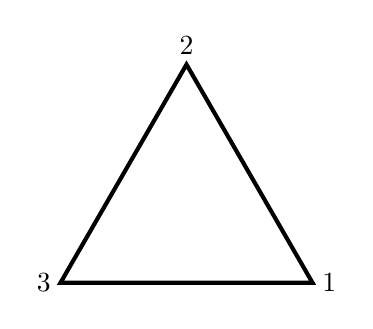
\begin{tikzpicture}[scale=0.8]
        \coordinate[label=left:$3$]  (A) at (0,0);
        \coordinate[label=right:$1$] (B) at (4,0);
        \coordinate[label=above:$2$] (C) at (2,3.464);
        
        \draw[line width=1.5pt] (A) -- (B) -- (C) -- cycle;
    \end{tikzpicture}
\end{center}

Given such a triangle, there are two main transformations we can make -- rotations and reflections. In total there are 6 such symmetries:
\begin{center}
    \begin{tabular}{ c c c }
        % Identity
        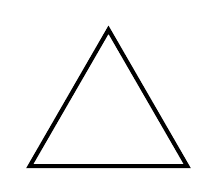
\begin{tikzpicture}
            \coordinate (A) at (0,0);
            \coordinate (B) at (2,0);
            \coordinate (C) at (1,1.732);
            
            \draw[line width=1.5pt] (A) -- (B) -- (C) -- cycle;
        \end{tikzpicture} 
        &
        % Left rotation
        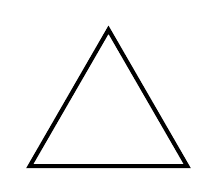
\begin{tikzpicture}
            \coordinate (A) at (0,0);
            \coordinate (B) at (2,0);
            \coordinate (C) at (1,1.732);
            
            \draw[line width=1.5pt] (A) -- (B) -- (C) -- cycle;
            
            % \draw[ultra thick, red, -{>[sep=2pt]}]
            %     (A) [left] edge [bend right=45] (B)
            %     (B) edge [bend right=45] (C)
            %     (C) edge [bend right=45] (A);
        \end{tikzpicture}
        &
        % Right rotation
        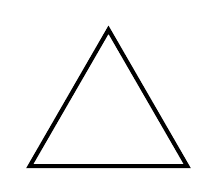
\begin{tikzpicture}
            \coordinate (A) at (0,0);
            \coordinate (B) at (2,0);
            \coordinate (C) at (1,1.732);
            
            \draw[line width=1.5pt] (A) -- (B) -- (C) -- cycle;
        \end{tikzpicture}
        \\
        % Top reflection
        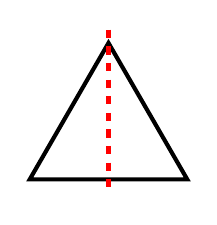
\begin{tikzpicture}
            \coordinate (A) at (0,0);
            \coordinate (B) at (2,0);
            \coordinate (C) at (1,1.732);
            
            \draw[line width=1.5pt] (A) -- (B) -- (C) -- cycle;

            \draw[red, dashed, line width=1.5pt] (1, 1.9) -- (1, -0.2);
        \end{tikzpicture}
        &
        % Left reflection
        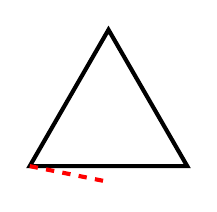
\begin{tikzpicture}
            \coordinate (A) at (0,0);
            \coordinate (B) at (2,0);
            \coordinate (C) at (1,1.732);
            
            \draw[line width=1.5pt] (A) -- (B) -- (C) -- cycle;

            \draw[red, dashed, line width=1.5pt] (0, 0) -- (1, -0.2);
        \end{tikzpicture}
        &
        % Right reflection
        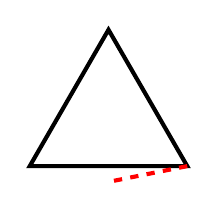
\begin{tikzpicture}
            \coordinate (A) at (0,0);
            \coordinate (B) at (2,0);
            \coordinate (C) at (1,1.732);
            
            \draw[line width=1.5pt] (A) -- (B) -- (C) -- cycle;

            \draw[red, dashed, line width=1.5pt] (2, 0) -- (1, -0.2);
        \end{tikzpicture}
    \end{tabular}
\end{center}

For each of these symmetries, we can compose or ``multiply'' them. For instance, we may perform a rotation followed by a reflection.

% Insert an image of three triangles to demonstrate composition

Firstly, notice that the result of two such composition is itself a symmertry. Specifically, it is the symmerty obtained by reflecting the trianlge by an axis that passes through the vertex $2$. There are three important features to note. 
\begin{enumerate}
    \item There is an identity (a symmetry that does nothing)
    \item Every symmetry has an inverse
    \item Symmerty multiplication is \emph{associative}
\end{enumerate}
Furthermore, there is an important non-feature; multiplication may not be commutative. In this case, performing a rotation followed by a reflection does not result in the same result as if the order of transformations were reversed. 

% Insert an image of three triangles to demonstrate non commutativity

\subsection{Algebra}

With the example in mind, we will now define what a group is algebraically. 

\begin{defi}[Binary Operation]
    A \emph{binary operation} on the set $X$ is a map
    \begin{align*}
        \cdot \ X \times X \rightarrow x \\
        (x, y) \longmapsto x \cdot y
    \end{align*}
\end{defi}

\begin{defi}[Group]
    A \emph{group} is a triple $(G, \cdot, e)$ where
    \begin{enumerate}
        \item $G$ is a set
        \item $\cdot$ is a binary operation
        \item $e \in G$
    \end{enumerate}

    Satisfying three Axioms
    \begin{enumerate}
        \item (Associativity) $\forall a, b, c \in G, \quad (a \cdot b) \cdot c = a \cdot (b \cdot c)$
        \item (Identity) $\forall a \in G, \quad a \cdot e = G$
        \item (Inverse) $\forall a \in G, \exists b \ \text{s.t.} \ a \cdot b = e$
    \end{enumerate}
\end{defi}

These axioms generalise the example encountered earlier.
\begin{eg}
    Consider the group $(\Z, +, 0)$

    We can show this forms a group as we have
    \begin{enumerate}
        \item (Associativity) since addition over the integers is associative
        \item (Identity) since $0$ acts as an additive identity
        \item (Inverse) since $\forall a \in \Z, \quad a + (-a) = 0$
    \end{enumerate}
\end{eg}
Now that we have established the axioms of groups we can prove some immediate properties.

\begin{prop}
    Let $(G, \cdot, e)$ be a group, and $a, b, b^{\prime}, e, e^{\prime} \in G$. Then,
    \begin{enumerate}
        \item if $a \cdot b = e$ then $b \cdot a = e$
        \item $e \cdot a = a$
        \item if $a \cdot b = e = a \cdot b^{\prime}$ then $b = b^{\prime}$
        \item if $a \cdot e^{\prime} = a$ then $e = e^{\prime}$
    \end{enumerate}
\end{prop}

\begin{proof}\leavevmode
    \begin{enumerate}
        \item We will show that inverses commute
        \begin{align*}
            b &= b \cdot e \tag{identity} \\
            &= b \cdot (a \cdot b) \tag{hypothesis} \\
            &= (b \cdot a) \cdot b \tag{associativity}
        \end{align*}

        By inverses, $\exists c \in G$ such that $b \cdot c = e$, so multiplying both sides of the equation on the right gives,

        \begin{align*}
            b \cdot c &= ((b \cdot a) \cdot b) \cdot c \\
            &= (b \cdot a) \cdot (b \cdot c) \tag{associativity} \\
            &= (b \cdot a) \cdot e \tag{identity}
        \end{align*}

        Hence, $e = b \cdot a$ as required
        
        \item We will show that left identity and the right identity are the same. By inverses and by part (i), $\exists b \in G$ such that $a \cdot b = e = b \cdot a$ 
        \begin{align*}
            e \cdot a &= (a \cdot b) \cdot A \\
            &= a \cdot (b \cdot a) \tag{associativity}\\
            &= a \cdot e \\
            &= a \tag{identity}
        \end{align*}

        \item We will show that multiplication is unique 
        \begin{align*}
            b^{\prime} &= e \cdot b^{\prime} \tag{ii}\\
            &= (b \cdot a) \cdot b^{\prime} \tag{i}\\
            &= b \cdot (a \cdot b^{\prime}) \tag{associativity}\\
            &= b \cdot e \tag{hypothesis} \\
            &= b \tag{identity}
        \end{align*}

        Alternatively, a for a stronger argument. $\exists c \in G$ such that $c \cdot a = e$
        \begin{align*}
            a \cdot b &= a \cdot b^{\prime} \\
            c \cdot (a \cdot b) &= c \cdot (a \cdot b^{\prime}) \\
            (c \cdot a) \cdot b &= (c \cdot a) \cdot b^{\prime} \tag{associativity} \\
            e \cdot b &= e \cdot b^{\prime} \\
            b &= b^{\prime} \tag{ii}
        \end{align*}

        \item We will show that identity is unique. By inverses and part (i), $\exists b \in G$ such that $b \cdot a = e$.
        \begin{align*}
            b \cdot a &= b \cdot (a \cdot e^{\prime}) \tag{hypothesis}\\
            &= (b \cdot a) \cdot e^{\prime} \tag{hypothesis}\\
            &= e \cdot e^{\prime} \\
            &= e^{\prime}
        \end{align*}
        
        Hence $e = e^{\prime}$
    \end{enumerate}
\end{proof}

%%%%%%%%%%%%%%%%%%%%%%
% Lecture 2: 7/10/2023
%%%%%%%%%%%%%%%%%%%%%%

Note that part (iii) says that inverses are \emph{unique}. Therefore, if $a \cdot b = e$. Firstly, we will introduce the superscript ``$-1$'' notation to indicate an inverse of some element. Then we can write
\begin{align*}
    b &= a^{-1} \\
    a \cdot a^{-1} &= e = a^{-1} \cdot a
\end{align*}

Therefore we have that the inverse of an inverse brings us back to the original element.
\[
    (a^{-1})^{-1} = a  
\]

Using this new notation, we can now define notation to write $\forall a \in G, \forall n \in \N$,
\begin{center}
    \begin{itemize}
        \item $a^0 = e$
        \item $a^1 = a$
        \item $a^2 = a \cdot a$
        \item[$\vdots$]
        \item $a^n = a^{n-1} \cdot a$
    \end{itemize}
\end{center}

We can also define negative exponentials as
\[
    a^n = (a^{-1})^{-n} \quad \text{for} \ n = -1, -2, -3, \ldots
\]

\begin{ex} Show that the following holds
    \begin{enumerate}
        \item $a^{m} \cdot a^{n} = a^{m + n}$
        \item $(a^{m})^{n} = a^{mn}$
    \end{enumerate}
\end{ex}
\begin{proof}\leavevmode
    \begin{enumerate}
        \item
        \begin{align*}
            a^m \cdot a^n &= a^m \cdot (a^{n-1} \cdot a) \tag{by definition} \\
            &= (a^m \cdot a) \cdot a^{n-1} \tag{associativity} \\
            &= a^{m+1} \cdot a^{n-1}
        \end{align*}

        Then we may proceed by induction, to arrive at
        \begin{align*}
            a^m \cdot a^n &= a^{m+n} \cdot a^{n-n} \\
            &= a^{m+n} \cdot a^0 \\
            &= a^{m+n} \cdot e \tag{by definition}\\
            &= a^{m+n} \tag{identity}
        \end{align*}
        
        \item
        \begin{align*}
            (a^m)^n &= (a^m)^{n-1} \cdot a^m \tag{by definition} \\
            &= ((a^m)^{n-2} \cdot a^m) \cdot a^m \\
            &= (a^m)^{n-2} \cdot (a^m \cdot a^m) \tag{associativity} \\
            &= (a^m)^{n-2} \cdot a^{2m} \tag{i} \\
        \end{align*}

        Then we may proceed by induction, to arrive at
        \begin{align*}
            (a^m)^n &= (a^m)^{0} \cdot a^{nm} \\
            &= e \cdot a^{nm} \tag{by definition} \\
            &= a^{nm} \tag{identity}
        \end{align*}
    \end{enumerate}
\end{proof}

\begin{remark}
    Recall that $a \cdot b$ is not necessarily $b \cdot a$ is a group $G$. So, we have to be careful when taking inverses after multiplying, the order of multiplication is reversed.
    \[
        (a \cdot b)^{-1} = b^{-1} \cdot a^{-1}  
    \]
\end{remark}

\begin{defi}[Abelian Group]
    If $(G, \cdot, e)$ is a group amd further satisfies that $a \cdot b = b \cdot a, \quad \forall a, b \in G$ then $G$ is called \emph{Abelian}
\end{defi}

\begin{defi}[Order of Group]
    The order of a group $(G, \cdot, e)$ is the number of elements of $G$, $\abs{G}$. If $\abs{G} < \infty$, then the group is finite
\end{defi}

\begin{eg}
    Here are some example and non-examples of groups
    \begin{enumerate}
        \item Trivial group. If $G = \{e\}$ and $e \cdot e = e$ then $(G, \cdot, e)$ is called the \emph{Trivial Group}
    \end{enumerate}
    Familiar examples from arithmetic
    \begin{enumerate}[resume]
        \item $(\Z, +, 0), (\Q, +, 0), (\R, +, 0), (\C, +, 0)$ as all abelian groups. In particular, the inverse of $x$ is $-x$
        \item $(\N, +, 0)$ is \emph{NOT} a group as there are no inverses
        \item $(\Q, \times, 1)$ is \emph{NOT} as group (0 does not have an inverse)
        \item $(\Q \setminus \{0\}, \times, 1), (\R \setminus \{0\}, \times, 1), (\C \setminus \{0\}, \times, 1)$ are abelian groups
    \end{enumerate}
    Finite examples
    \begin{enumerate}[resume]
        \item $\forall n \in \N, \ \text{let} \ C_n = \{z \in \C \mid z^n = 1\}$. Then $(c_n, \times, 1)$ forms an abelian group of order $n$
        \item Let $\Z_n = \{a \in \N \cup \{0\} \mid a < n\}$. Then for $a, b \in \Z_n$, let $a +_n b$ be the remainder when $a + b$ is divided by $n$. Then $(\Z_n, +_n, 0)$ form a group.
    \end{enumerate}
\end{eg}

%%%%%%%%%%%%%%%%%%%%%%
% Lecture 3: 10/10/2023
%%%%%%%%%%%%%%%%%%%%%%

\subsection{Matrix Groups}
\begin{defi}[Matrix Group]
    Let $GL_2(\R)$ be the set of all $2 \times 2$ matrices
    \[
        A = \begin{pmatrix}
            a & b \\
            c & d
        \end{pmatrix} \quad \text{with} \quad a,b,c,d \in \R
    \]
    and $A$ is invertible i.e; $A$ has an inverse. $\exists B \in GL_2$ such that
    \[
        AB = \begin{pmatrix}
            1 & 0 \\
            0 & 1
        \end{pmatrix}
    \]
    Then $(GL_2(\R), \cdot, \begin{pmatrix}
        1 & 0 \\
        0 & 1
    \end{pmatrix})$ form a group
\end{defi}

From this definition we can see that this group is non-abelian -- as matrix multiplication is non-commutative, and that the group is infinite. For example, consider matrices of the form
\[
    \begin{pmatrix}
        1 & t \\
        0 & 1
    \end{pmatrix} \quad \forall t \in \R
\]

\subsection{Symmetric Groups}
\begin{defi}[$\Sym(X)$]
    Let $X$ be a set. Then we define $\Sym(X)$ to be the set of all bijections from $X \rightarrow X$. Alternatively we can think of this set as being the same as the set of all permutations of $X$.
\end{defi}

\begin{defi}[$\Id_x$]
    The identity map, $\Id_x$ is defined as the map $x \mapsto x$. 
\end{defi}

\begin{lemma}[Compositive is associative]
    Consider maps $f, g, h$ of sets $w, x, y, z$
    \begin{center}
        \begin{tikzpicture}
            \graph {
                w ->["f"] x ->["g"] y ->["h"] z;
            };
        \end{tikzpicture}
    \end{center}
    Then $(h \circ g) \circ f = h \circ (g \circ f)$
\end{lemma}

\begin{proof}
    We will watch what happens to an element over the composed maps. Let $w \in W$
    \begin{align*}
        (h \circ g) \circ f (w) &= (h \circ g)(f(w)) \\
        &= h(g(f(w))) \\
        &= h(g \circ f(w)) \\
        &= h \circ (g \circ f)(w)
    \end{align*}
\end{proof}

\begin{prop}
    For any set $X, (\Sym(x), \circ, \Id_x)$ form a group
\end{prop}

\begin{proof}[Symmetric Group]
    To prove that $(\Sym(x), \circ, \Id_x)$ forms a group we need to show that
    \begin{enumerate}
        \item Associativity follows from the Lemma
        \item $\Id_x$ is the identity
        \item Inverses exist by the definition of bijection
    \end{enumerate}
\end{proof}

We are particularly interested in cases where $X$ is finite.
\begin{defi}[$S_n$]
    If $x = {1, 2, \cdots, n}$ then $S_n \equiv \Sym(X)$
\end{defi}

\begin{ex}
    What is the order of $S_n$?
\end{ex}

\begin{proof}
    The order of $S_n$ is equal to the number of permutations of $n$ elements and therefore $n!$
\end{proof}

\begin{remark}
    Before moving on, let's take note of the notation we are using. Currently, it takes a triple $(G, \cdot, e)$ to define a group. Moving forward, we will simply write $G$ to represent the whole group. However, when dealing with multiple groups, we will use $\cdot_G$ and $e_G$ to specify which binary operation and which identity belongs to the group $G$.
\end{remark}

\subsection{Subgroups}
\begin{defi}[Subgroup]
    Let $(G, \cdot_G, e_G)$ and $(H, \cdot_H, e_H)$ be groups. If
    \begin{enumerate}
        \item $H \subseteq G$
        \item $e_H = e_G$
        \item $\forall a, b \in H, \quad a \cdot_H b = a \cdot_G b$
    \end{enumerate}
    then $H$ is a \emph{subgroup} of $G$ and we write $H \leq G$
\end{defi}

\begin{prop}[Subgroup Criterion]
    Let $G$ be a group and $H \subseteq G$ be a non-empty subset. If
    \[
        \forall a, b \in H, \quad a \cdot_G b^-1 \in H
    \]
    then $H \leq G$
\end{prop}

\begin{proof}
    Since $H$ is nonempty, let $x \in H$. Therefore assuming the subgroup criterion,
    \begin{enumerate}
        \item (Identity) $x \cdot_G x^{-1} \in H \Rightarrow e_G \in H$
        \item (Inverse) $e_G \cdot_G a^{-1} \in H \Rightarrow a^{-1} \in H \quad \forall a \in H$
        \item (Closure) \begin{align*}
            \forall a, b \in H, b^{-1} \in H \tag{by Inverse} &\Rightarrow a \cdot_G (b^{-1})^{-1} \in H \\
            &\Rightarrow a \cdot_G b \in H
        \end{align*}
    \end{enumerate}
    Finally, if we set $\cdot_H =$ ``restriction of $\cdot_G$'' to $H$ and $e_H = e_G$ then $H \leq G$. 
\end{proof}

\begin{eg}\leavevmode
    \begin{enumerate}
        \item Every group $G$ is a subgroup of itself
        \item For every group $G$, $I_G = \{e_G\}$ is the Trivial subgroup
    \end{enumerate}
    Propper subgroups
    \begin{enumerate}[resume]
        \item $\Z \leq \Q \leq \R \leq \C$
        \item If $H_i \leq G$ for some set of $i$ then
        \[
            H = \bigcap_{i}{H_i} \leq G   
        \]
        is a subgroup.
        \item For any subset $X \subseteq G$, define
        \[
            \anglebk{X} = \bigcap_{X \subseteq H \leq G}{H} \leq G
        \]
        This is known as the subgroup \emph{generated} by $X$. In the case that $\anglebk{X} = G$ we say that $X$ \emph{generates} $G$
    \end{enumerate}
\end{eg}

\begin{ex}[Intersection of Subgroups]
    Prove statement (iv) that the intersection of subgroups is itself a subgroup. 
\end{ex}

\begin{proof}
    We will proceed by contradiction. Consider two elements $a, b \in H$. Since $H$ is the intersection of all $H_i$, $a, b \in H_i $ for all $i$.
    
    Suppose $b^{-1} \notin H$. Then, $\exists i$ such that $b^{-1} \notin H_i$. However, $H_i$ is a subgroup that fulfils the subgroup criterion. This is a contradiction \contradiction.

    Define $c \equiv a \cdot b^{-1}$. Suppose $c \notin H$. Then $\exists i$ such that $c \notin H_i$. However $H_i$ is a subgroup and must contain $c$ since it contains both $a$ and $b$. This is a contradiction \contradiction.
    
    Hence, $\forall a,b \in H, \quad a \cdot b^{-1} \in H \Rightarrow H \leq G$
\end{proof}

\begin{prop}
    The subgroups of $\Z$ are exactly the subsets
    \[
        n\Z = \{nk \in \Z \mid k \in \Z\} \quad \forall n = 0, 1, 2, \ldots
    \]
\end{prop}

%%%%%%%%%%%%%%%%%%%%%%
% Lecture 4: 12/10/2023
%%%%%%%%%%%%%%%%%%%%%%

\begin{proof}
    Note that each $n\Z$ is a subgroup of $\Z$. Applying the subgroup criterion, if
    \[
        a = nk, \quad b = nl \quad \text{for} \ k, l \in \Z  
    \]
    Then,
    \[
        a - b = n(k - l) \in n\Z  
    \]
    therefore each of $n\Z \leq Z$.

    Now suppose that for some subgroup $H \leq Z$. 
    If $H = \{0\}$, then $H = 0\Z$ and we have shown $H$ to be of the form $n\Z$.
    Otherwise, $H \neq \{0\}$ and we may choose some $n \in H \setminus \{0\}$ to be the smallest positive element of $H$. Since $H$ is closed under inverses,
    \[
        -n \in H  
    \]
    Since $H$ is closed under addition,
    \begin{align*}
        n + n = 2n &\in H \\
        2n + n = 3n &\in H \\
        &\vdots \\
        \forall k \in \Z^+, \ kn &\in H 
    \end{align*}
    Further,
    \begin{align*}
        -n - n = -2n &\in H \\
        -2n - n = -3n &\in H \\
        &\vdots \\
        \forall k \in \Z^-, \ kn &\in H 
    \end{align*}
    Therefore
    \[
        n\Z \leq H  
    \]
    We now want to show that $n\Z = H$. We will proceed by contradiction. Suppose $n\Z \neq H$, then $\exists x \in H$ such that $x \notin n\Z$. Using the division algorithm we can write
    \[
        x = nq + r, \quad \text{for} \ q \in \Z, \ 0 < r < n-1  
    \]
    Note that $r$ cannot be $0$ if not $x$ would belong in $n\Z$. Therefore
    \[
        r = x - qn  
    \]
    Note that since $x \in H$ and $qn \in H$, $r \in H$. However, $r$ would also be smaller than $x$. This is a contradiction \contradiction.
\end{proof}

\subsection{Geometric Examples}

Let $\C$ be the comoplex plane, equipped with the usual notaion of distance.

% insert diagram of complex plane

\begin{defi}[Isometry]
    For any subset $X \subseteq \C$, an \emph{isometry} of $X$ is an bijecetion $f: X \rightarrow X$ that preserves distance:
    \[
        \abs{f(x) - f(y)} = \abs{x - y}, \quad \forall x, y \in X
    \]
\end{defi}

\begin{prop}[Isometry Groups in $\C$]
    Let $X \subseteq \C$. The set of isometries of $X$,
    \[
        \Isom(X) = \{f: X \rightarrow X \mid f \ \text{is a bijection \& isometry}\}
    \]
    Then $\Isom(X)$ is a group with function composition and the identity map and it is a subgroup of $\Sym(X)$.
\end{prop}

\begin{proof}
    Since $\Id_x \in \Isom(X)$, $\Isom(X)$ is non-empty. By the subgroup criterion, it suffices to check that
    \[
        f \circ g^{-1} \in \Isom(X), \quad \text{for} \ f, g \in \Isom(X)   
    \]
    Let $x, y \in X$. Then,
    \begin{align*}
        \abs{f \circ g^{-1}(x) - f \circ g^{-1}(y)} &= \abs{g^{-1}(x) - g^{-1}(y)} \\
        &= \abs{g \circ g^{-1}(x) - g \circ g^{-1}(y)} \\
        & = \abs{x - y}
    \end{align*}
\end{proof}

\begin{defi}[Dihedral Groups]
    Let $X_n \subset \C$ be the $n$-gon with vertices written
    \[
        X_n = \{e^\frac{2\pi i k}{n} \mid k = 0, 1, \ldots, n-1 \}, \quad \text{for} \ n\geq 3
    \]
    Then we define the $n^{th}$ dihedral group as follows: (note the notation of using $2n$)
    \[
        \D_{2n} \equiv \Isom(X_n)
    \]
\end{defi}

\begin{eg}
    $\D_6$ is the isometry group of the equilateral triangle, and $\abs{\D_6} = 6$ 
\end{eg}

\begin{thm}[$\abs{\D_{2n}} = 2n$]
\end{thm}

We will first prove some lemmas from geometry

\begin{lemma}[Kite lemma]
    Let $x_1, x_2, y_1, y_2 \in \C$. If
    \begin{align*}
        \abs{y_1 - x_1} &= \abs{y_2 - x_1} \\
        \abs{y_1 - x_2} &= \abs{y_2 - x_2}
    \end{align*}
    Then, $x_2 - x_1$ is perpendicular to $y_2 - y_1$
\end{lemma}

\begin{proof}
    Excercise!
\end{proof}

\begin{lemma}[Kite lemma]
    Let $x \subset \C$ and $f \in \Isom(x)$. If there are three points $x_1, x_2, x_3$ that are not colinear such that
    \[
        f(x_1) = x_1, \quad f(x_2) = x_2, \quad f(x_3) = x_3  
    \]
    then $f = \Id_x$
\end{lemma}
\begin{proof}
    We will proceed by contradiction. Suppose $\exists y \in X$ such that $f(y) \neq y$. Then,
    \begin{align*}
        \abs{f(y) - x_i} &= \abs{f(y) - f(x_i)} \\
        &= \abs{y - x_i}
    \end{align*}
    which will be true for $i = 1, 2, 3$.

    Let $y_1 = y$, and $y_2 = f(y)$. Then by the Kite lemma,
    \begin{align*}
        x_2 - x_1 &\perp f(y) - y \neq 0 \\
        x_3 - x_1 &\perp f(y) - y \neq 0
    \end{align*}
    Therefore, $x_1, x_2, x_3$ are colinear which is a contradiciton. \contradiction
\end{proof}

We will now show a stronger version, of the theorem stated earlier,
\begin{thm}[$\abs{\D_{2n}} = 2n$]
    If we define 2 elements in $\D_{2n}$
    \begin{enumerate}
        \item $r(z) = e^\frac{2 \pi i}{n} \cdot z$
        \item $s(z) = \overline{z}$
    \end{enumerate}
    Then,
    \[
        \D_{2n} = \{e, r, r^2, \ldots, r^{n-1}, s, rs, \ldots, r^{n-1}s\}  
    \]
\end{thm}
\end{document}